\documentclass[crop,tikz]{standalone}

\tikzset{>=latex}
\usetikzlibrary{shapes}
\colorlet{gray}{gray!50}

\begin{document}
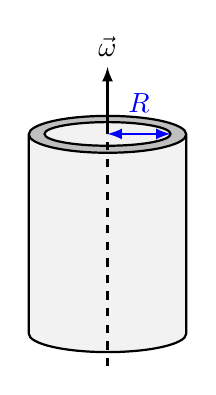
\begin{tikzpicture}
  % thin cylinder
  \node (Z) at (0,0) [thick, cylinder, aspect=2, shape border rotate=90, draw, minimum height=3cm, minimum width=2cm, cylinder body fill=gray!20, cylinder uses custom fill, cylinder end fill=gray] {};
  \draw[thick,fill=gray!20] (0,1.45) ellipse (0.8 and 0.15);
  % rotation axis
  \draw[dashed,thick] (0,-1.5) -- +(0,3);
  \draw[->,thick] (0,1.5) -- +(0,0.8) node[above] {$\vec{\omega}$};
  % radius
  \draw[<->,thick,blue] (0,1.45) -- node[above,yshift=0.4em] {$R$} +(0.8,0);
\end{tikzpicture}
\end{document}
